\documentclass[conference, letterpaper, 10pt, times]{IEEEtran}

%% IEEE CNS addition:
\makeatletter
\def\ps@headings{%
	\def\@oddhead{\mbox{}\scriptsize\rightmark \hfil \thepage}%
	\def\@evenhead{\scriptsize\thepage \hfil \leftmark\mbox{}}%
	\def\@oddfoot{}%
	\def\@evenfoot{}}
\makeatother
\pagestyle{empty}

\usepackage[T1]{fontenc}

\usepackage[dvipsnames]{xcolor}
\usepackage{graphicx}

\usepackage[binary-units]{siunitx}
\sisetup{range-phrase=--, range-units=single}

\usepackage[basic]{complexity}
\usepackage[super,negative]{nth}

\usepackage{booktabs}
\usepackage{microtype}

%% Fix indent in new section...
\newcommand{\subparagraph}{}
\usepackage{titlesec}
\titlespacing*{\section}{0pt}{1.5ex}{0.7ex}
%\titleformat*{\filcenter\scshape}

%bib
\usepackage[maxnames=3,maxbibnames=99,mincrossrefs=5,style=ieee,sortcites,backend=bibtex]{biblatex}
%\addbibresource{papers-off.bib}
%\addbibresource{confs-off.bib}
%\addbibresource{rfc.bib}

%picky abt et al.
\usepackage{xpatch}

\xpatchbibmacro{name:andothers}{%
	\bibstring{andothers}%
}{%
	\bibstring[\emph]{andothers}%
}{}{}

%opening!

\newcommand{\mytitle}{Improving Direct-Control Reinforcement Learning for Network Intrusion Prevention}

\usepackage{url}
\usepackage{hyperref}
\usepackage{cleveref}
\newcommand{\crefrangeconjunction}{--}

\hypersetup{
	colorlinks,
	citecolor=black,
	filecolor=black,
	linkcolor=black,
	urlcolor=black,
	pdftitle={\mytitle{}},
	pdfauthor={Kyle A. Simpson}
}
\newcommand*{\email}[1]{\href{mailto:#1}{\nolinkurl{#1}} } 

\usepackage{titling}
\settowidth{\thanksmarkwidth}{*}
\setlength{\thanksmargin}{-\thanksmarkwidth}

%% Enable /thanks
\IEEEoverridecommandlockouts
\makeatletter
\def\footnoterule{\relax%
	\kern-5pt
	\hbox to \columnwidth{\hfill\vrule width 0.5\columnwidth height 0.4pt\hfill}
	\kern4.6pt}
\makeatother

%-------------------------------------%
%-------------------------------------%

\title{\mytitle{}}
\author{Kyle A. Simpson\thanks{This work was supported by the Engineering and Physical Sciences
		Research Council [grant number EP/M508056/1]}\\\emph{University of Glasgow, Glasgow, Scotland},\\
		\email{k.simpson.1@research.gla.ac.uk}}

% Remove date, leave no spacing.
\predate{}
\postdate{}
\date{}

\begin{document}

%% If needed, make urls typewritery
%\urlstyle{tt}

\maketitle

\begin{abstract}
	Make it look convincing!
\end{abstract}

\section{Introduction}

What is the story I'm trying to push?

?? Threat model yada yada everything sucks all the time here are some statistics about things being 

?? Reference to the possible mistreatment of RL in our domain? The problem of ``blind application'' so hated by Sommer and Paxson.

?? RL as a mechanism to protect systems by monitoring performance characteristics---overcome the detection problem (different handle on the key problems of burstiness, evolution, non-stationarity).

This paper contributes:
\begin{itemize}
	\item A DDoS mitigation system based on direct-control reinforcement learning designed for deployment in real-world software-defined networks.
	\item Important weaknesses and flaws in the past design and evaluation of similar techniques.
	\item ?? Advancing the use/representation of state-space in direct-control RL of networked applications.
\end{itemize}

\section{Background}

?? Introduce RL, related definitions etc.

?? Is this \emph{actually} just sarsa? We're using fn approx (of course), but this is fraught with its own difficulties. Is it strictly speaking correct to describe it as Sarsa at this point? It's, at the very least, 1-step semi-gradient Sarsa given that it is clearly on-policy...
?? IDEA: try out average reward, td-$\lambda$ methods...

?? Discuss mininet? Networking terms?

\section{A Plan, of Sorts}

\begin{enumerate}
	\item The main case for contribution in what I have so far:
	\begin{itemize}
		\item Past work reliant on unrealistic network models: tcp-like behaviour (and its effects on collateral damage) not captured, disjoint ranges of traffic distribution (no benign heavy-hitters).
		\item I offer more realistic network emulation environment, better treatment of protocol/traffic characteristics.
	\end{itemize}
	\item Forthcoming: rethinking state/action spaces to operate at a finer level of granularity. New network model (live tcp back-and-forth), allows us to test collateral damage assumptions in a more realistic manner (and show clear case for moving beyond work of malialis and kudenko)
\end{enumerate}

\section{Results and Evaluation}

\begin{figure}[ht]
	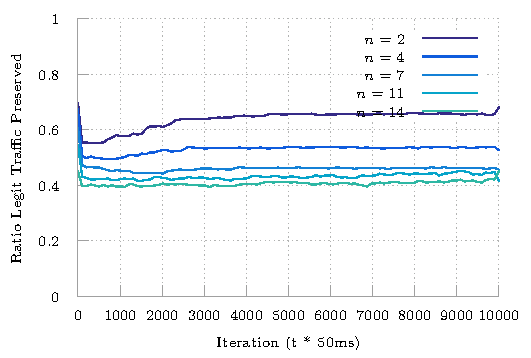
\includegraphics[width=\linewidth]{../plots/online-varyN-uneven}
	\caption{
		MARL pushback control system performance plotted over time, for various settings of $n$ hosts per learner.
		This plot shows that, from the perspective of benign hosts, service guarantees degrade as inference and applied actions become less granular.
		This generalises for all behavioural discriminators: even a perfect agent \emph{must} punish benign flows if they are grouped with malicious actors.
		\label{fig:marl-granularity}
	}
\end{figure}

See above: a result.

?? Observations: training time lengthier by nature of emulated environment.
?? Risk of going for a simulation (i.e. numeric)? Always going to be interesting behaviour that is missed out on (in theory), at the cost of training time/limits of simulation speed

\section{Related Work}

This is a new, modern paper, and so I acknowledge others \emph{after} myself.
How modest!

?? Abuses of RL

?? Direct-control work

?? Indirect-control applications: link to all the juicy stuff in e.g. HotNets, data-driven networking, the works. 

\section{Conclusion}

It all ends here, Mr.\ Bond...

?? Please write me once everything else is in place.

?? Future Work? I.e., \emph{everything}: no one else is really looking at/interested in this specific kind of application of RL yet. \emph{Yet}.

\section*{Acknowledgements}
My thanks go to Dr.\ Dimitrios Pezaros for his supervision, guidance, and comments relating to the realisation of this work.
Additional thanks \emph{would} go out to my anonymous reviewers, had I any of them.

\printbibliography

\end{document}